\documentclass{homework}
\usepackage{homework}
\usepackage{hanhua}
\title{report}
\subtitle{week 8}
\begin{document}

\maketitle
\section{findValue.h}
\subsection{函数说明}
在稀疏矩阵中找到相应坐标的元素
\paragraph{输入}
一个指向待查找的稀疏矩阵指针*t,两个整型i,j分别表示待查找的行和列。
\paragraph{输出}
一个元素类型,即在该稀疏矩阵T中相应坐标上所找到的的元素T[i][j]。若未找到则返回0。
\paragraph{实现方法}
依次扫描稀疏矩阵的元素,利用元素关于先行后列的字典序排列的性质,先跳到行号不小于所查找行位置的第一个元素,然后继续向后查找行号列号均相等的位置,返回其元素值。期间若有任何闪失均返回0。
\subsection{复杂度}
\paragraph{时间复杂度}
$\mathcal{O}(n) ~ n$为稀疏矩阵元素个数
\paragraph{空间复杂度}
$\mathcal{O}(1)$
\subsection{边界情况}
\begin{itemize}
    \item 传入空稀疏矩阵指针将得到0;
    \item 查找行列号为负数或超过指定稀疏矩阵的行列数将得到0;
    \item 注:所查找位置为从0开始的下标。
\end{itemize}
\subsection{程序运行结果}
\begin{figure}[H]
    \centering
    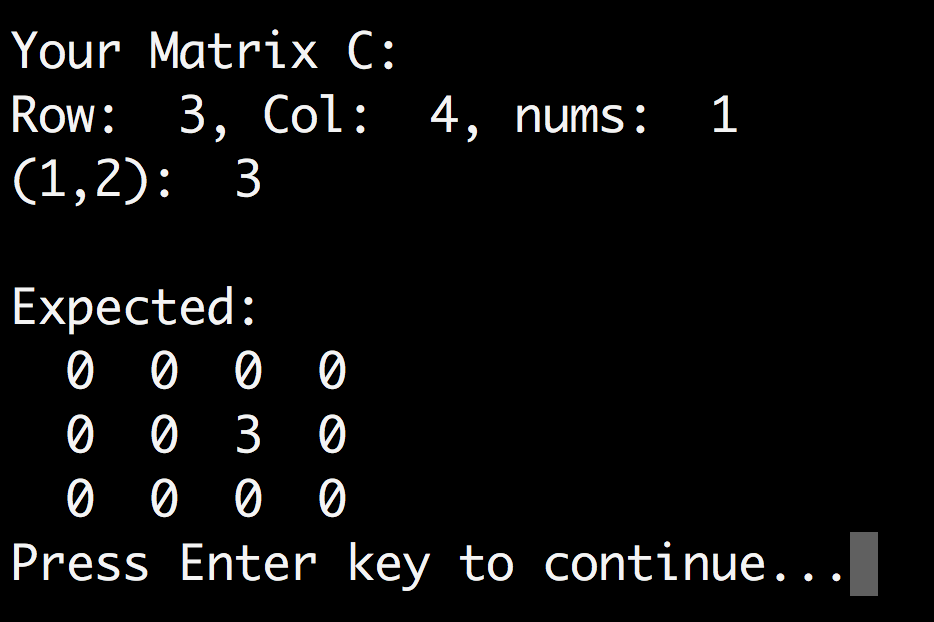
\includegraphics[width=7cm]{fig1.png}
\end{figure}
\section{multiMat.h}
\subsection{函数说明}
计算两个稀疏矩阵的乘积并以稀疏矩阵形式返回。
\paragraph{输入}
指向两个稀疏矩阵的指针*matA, *matB。
\paragraph{输出}
指向运算结果的稀疏矩阵指针*matC。
\paragraph{实现方法}
在输入矩阵可以相乘的情况下,声明一个正常的矩阵C,在进行完之后的累加以后将C转换为稀疏矩阵输出。

只有A(第一个矩阵)中列号与B(第二个矩阵)中行号相等的元素才会被乘到一起再累加到相应位置。依次扫描A中每个元素,对每个元素$a_{ij}$将能乘到一起的B中元素$b_{jk}$找到后相乘再累加到矩阵C的相应位置$c_{ik}$。

但对于$a_{ij}$若对每一个$0\leqslant$k<matB$\to$colSize都用前面的findValue函数查找一下$b_{jk}$,复杂度将达到$\mathcal{O}(N_AN_BZ)$,其中$N_A,N_B$分别为矩阵A和B中元素个数,$Z$为B的列数。

所以我们先对B进行预处理,利用元素行号单调递增的特性,将每一行第一个元素在元素列表中的位置标记出来bH[r]=$n_r,~0\leqslant r\leqslant Y,Y$为B的行数A的列数。若某行没有元素则仍标记为其后第一个元素位置,也就是每一行存储着行号不大于它的第一个元素的位置。对于不存在$Y+1$行即bH[Y]则存储元素总数。这样所有上下界形式一致了,B中第j行的所有元素b在元素列表中位置n满足bH[j]$\leqslant$n<bH[j+1],其中0$\leqslant$j<Y。

进行完预处理后,可以对于每个$a_{ij}$直接找到所有可乘的$b_{jk}$,将时间复杂度降到$\mathcal{O}(N_AN_B)$
\subsection{复杂度}
\paragraph{时间复杂度}
$\mathcal{O}(N_AN_B+Y+XZ),~X$为A的行数

$N_AN_B$为计算乘积时间,$Y$为预处理B所需时间,$XZ$为将C转换为稀疏矩阵存储形式时间。
\paragraph{空间复杂度}
$\mathcal{O}(Y+XZ)$
\subsection{边界情况}
\begin{itemize}
    \item 若有输入的稀疏矩阵指针为NULL,则返回NULL;
    \item 若两个矩阵不能相乘,则返回NULL;
    \item 若有矩阵的行或列不为正,则返回NULL;
    \item 若乘积结果是零矩阵,由于在声明矩阵C时使用calloc已经全部初始化为0元素了,结果正确。
\end{itemize}
\subsection{程序运行结果}
\begin{figure}[H]
    \centering
    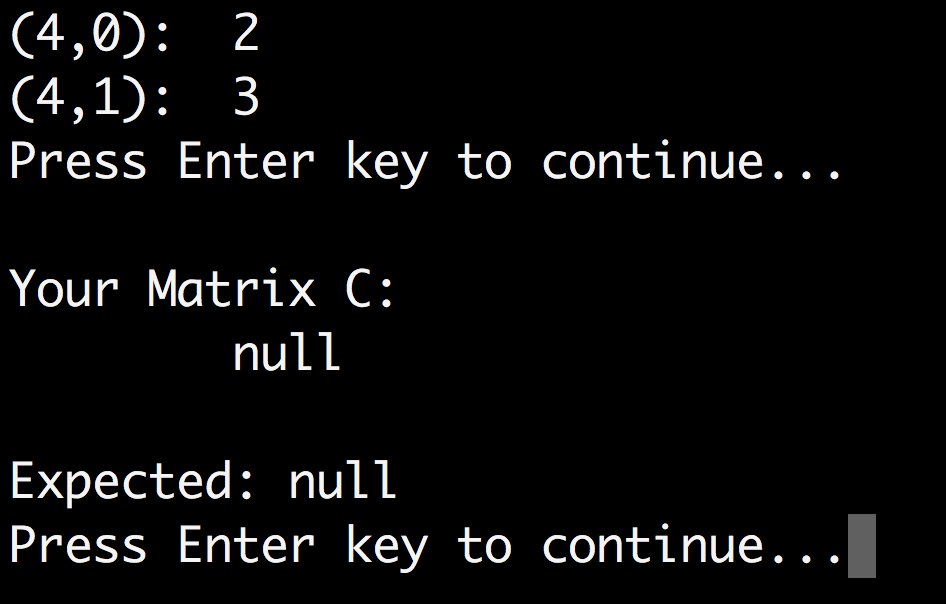
\includegraphics[width=7cm]{fig2.png}
\end{figure}
\end{document}
